	\begin{mydef}
		Si une figure et son symétrique par rapport à une droite $(d)$ sont confondus, alors $(d)$ est une axe de symétrie de la figure.
	\end{mydef}

	\begin{myexs}
		\begin{center}
			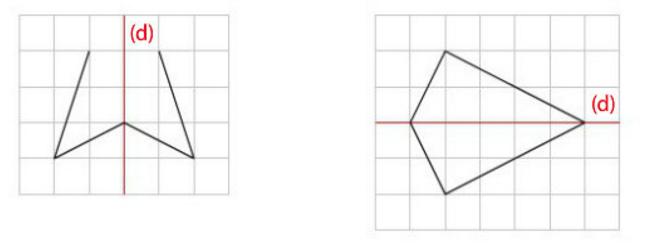
\includegraphics[scale=0.7]{axes}
		\end{center}
	\end{myexs}

	\begin{mydef}
		Si une figure et son symétrique par rapport à un point $O$ sont confondus, alors $O$ est un centre de symétrie de la figure.
	\end{mydef}

	\begin{myexs}
		\begin{center}
			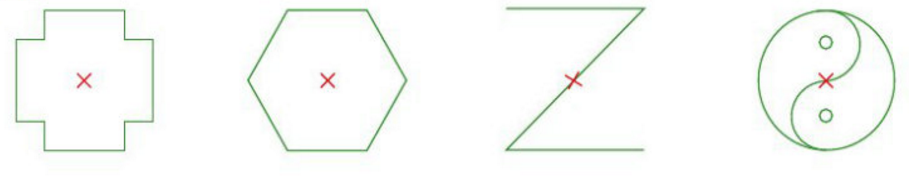
\includegraphics[scale=0.6]{centres}
		\end{center}
	\end{myexs}


	\begin{myapp}
		Dire si les panneaux suivants ont un axe et / ou un centre de symétrie.
		
		\begin{center}
			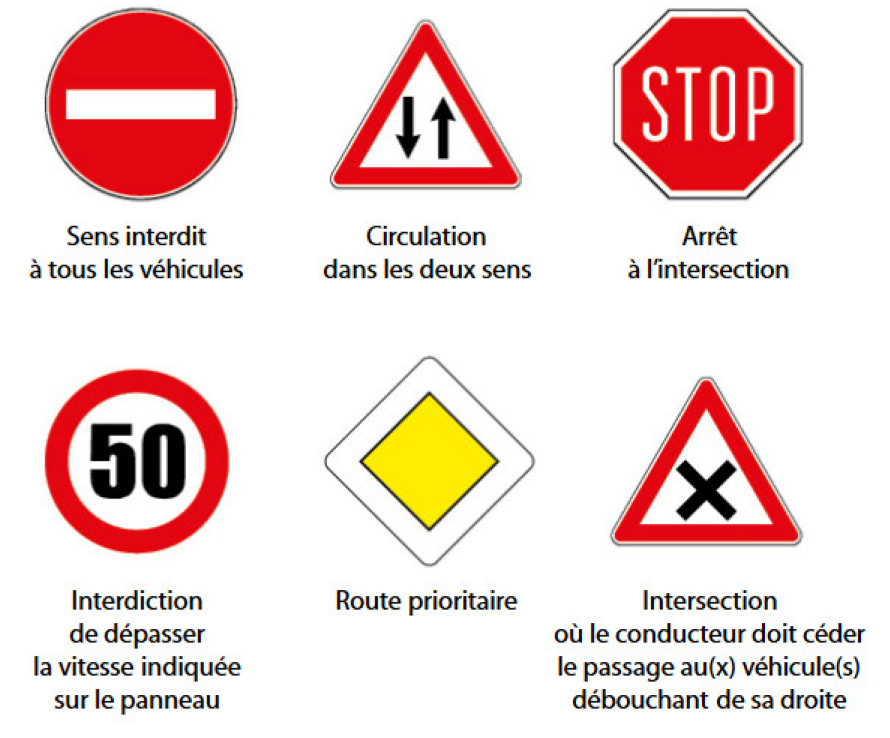
\includegraphics[scale=0.43]{app}
		\end{center}
	\end{myapp}